\chapter{Acides, bases et pH}\label{ch:g9:acids-bases-ph}

Sur une étagère de cuisine se trouvent un citron, une bouteille de
vinaigre, un savon et une boîte de bicarbonate de soude~; sous l'évier,
un flacon de déboucheur avec une étiquette d'avertissement noir et
rouge. Certains ont un goût acide, d'autres sont glissants au toucher,
d'autres peuvent brûler la peau. Une seule échelle, graduée de 0 à 14,
les classe tous --- et la même échelle sert pour les piscines, la terre
du jardin, le sang et les océans.

\begin{recall}
Les \omterm{def:g9:ions:ion}{ions} sont des \omterm{def:g7:atoms-and-molecules:atom}{atomes} ou des groupes d'\omterm{def:g7:atoms-and-molecules:atom}{atomes} porteurs d'une
charge~; un \omterm{def:g9:ions:ion}{cation} comme \ce{Na+} est positif, un \omterm{def:g9:ions:ion}{anion} comme \ce{Cl-}
ou \ce{OH-} négatif. Les solutions ioniques contiennent des \omterm{def:g9:ions:ion}{ions} notés
(aq), qui se déplacent librement (\cref{ch:g9:ions}).
\end{recall}

\begin{omfigure}
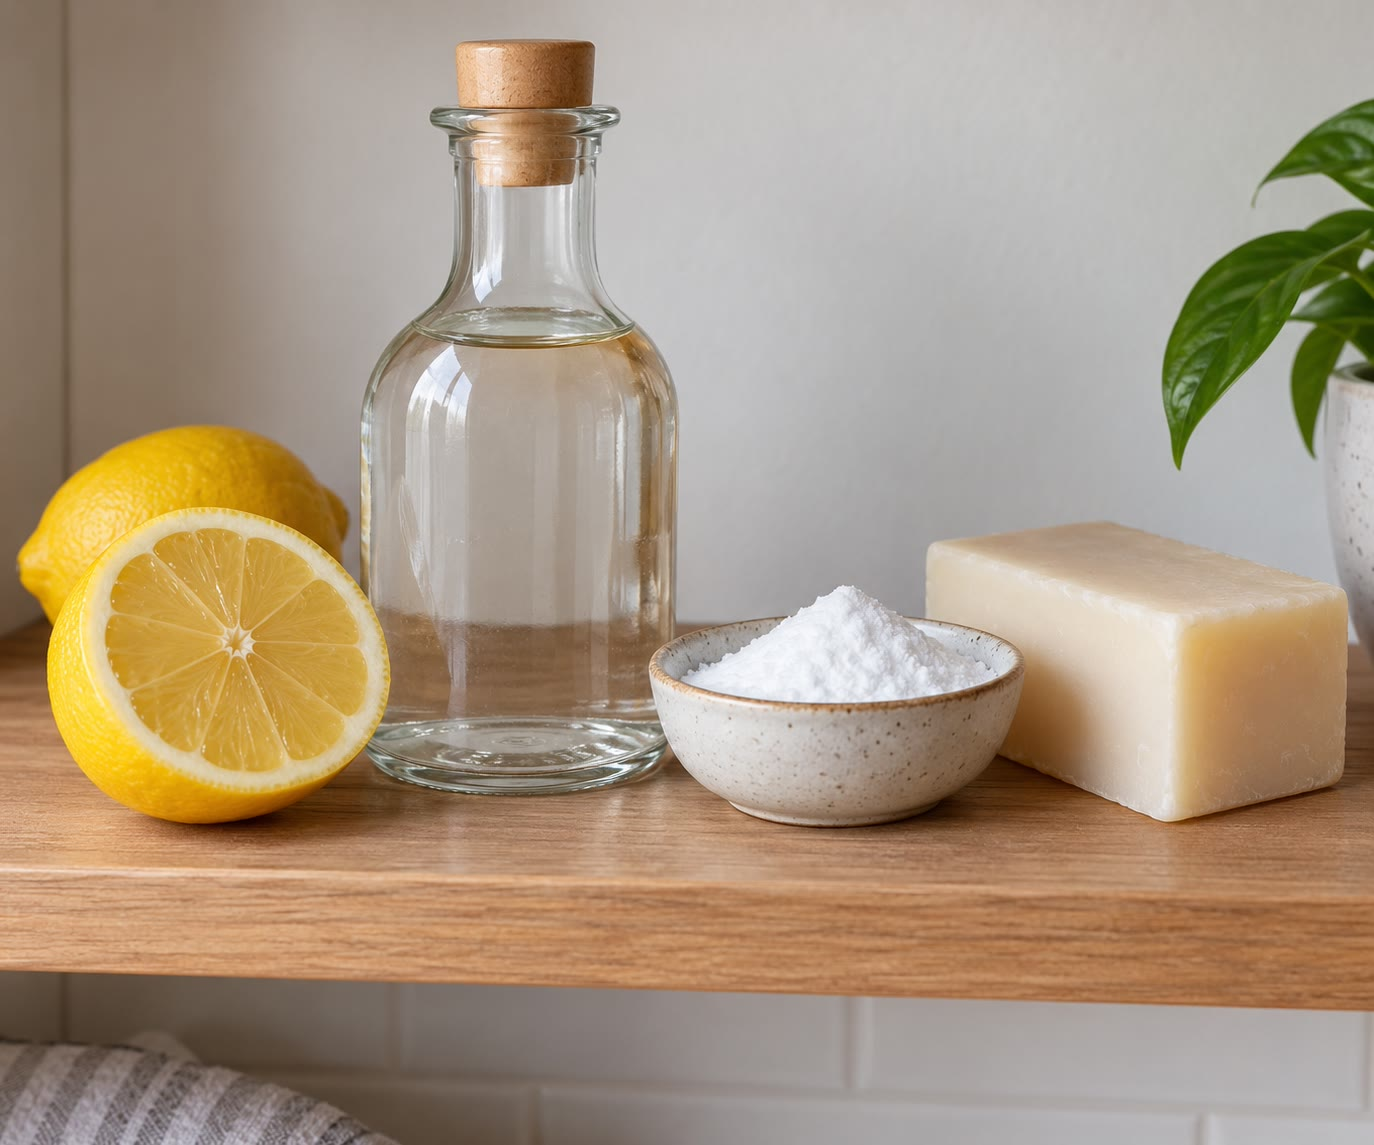
\includegraphics[width=0.55\linewidth]{images/book1/ai/g9-kitchen-shelf.jpg}

{\small Citron, vinaigre, savon et bicarbonate de soude~: des acides et
des bases dans la cuisine.}
\end{omfigure}

\section{Solutions acides, basiques et neutres}

\begin{definition}[Solutions acides, basiques et neutres]\label{def:g9:acids-bases-ph:acidic}
Toute \omterm{def:g6:solutions-and-solubility:solute}{solution aqueuse} contient des \omterm{def:g9:ions:ion}{ions} hydrogène \ce{H+(aq)} et des
\omterm{def:g9:ions:ion}{ions} hydroxyde \ce{OH-(aq)}. Une solution est une
\emph{solution acide}\index{solution acide} quand elle contient plus
d'\omterm{def:g9:ions:ion}{ions} \ce{H+} que d'\omterm{def:g9:ions:ion}{ions} \ce{OH-}, une
\emph{solution basique}\index{solution basique} quand elle contient plus
d'\omterm{def:g9:ions:ion}{ions} \ce{OH-} que d'\omterm{def:g9:ions:ion}{ions} \ce{H+}, et une \emph{solution
neutre}\index{solution neutre} quand elle en contient autant des uns que
des autres.
\end{definition}

\begin{example}[Trois solutions]\label{ex:g9:acids-bases-ph:three}
L'acide chlorhydrique est une \omterm{def:g9:acids-bases-ph:acidic}{solution acide}~: elle contient des \omterm{def:g9:ions:ion}{ions}
\ce{H+(aq)} et \ce{Cl-(aq)}, avec très peu d'\omterm{def:g9:ions:ion}{ions} \ce{OH-}. Une
solution d'hydroxyde de sodium est basique~: \ce{Na+(aq)} et
\ce{OH-(aq)}, avec très peu d'\omterm{def:g9:ions:ion}{ions} \ce{H+}. L'eau pure et l'eau salée
sont neutres.
\end{example}

\section{L'échelle de pH}

\begin{definition}[pH]\label{def:g9:acids-bases-ph:ph}
Le \emph{pH}\index{pH} d'une \omterm{def:g6:solutions-and-solubility:solute}{solution aqueuse} est un nombre, en général
compris entre 0 et 14, qui indique à quel point elle est acide ou
basique~: à \qty{25}{\celsius}, une \omterm{def:g9:acids-bases-ph:acidic}{solution neutre} a un pH égal à 7,
une \omterm{def:g9:acids-bases-ph:acidic}{solution acide} un pH inférieur à 7, une \omterm{def:g9:acids-bases-ph:acidic}{solution basique} un pH
supérieur à 7. Plus une solution contient d'\omterm{def:g9:ions:ion}{ions} \ce{H+}, plus son pH
est bas.
\end{definition}

\begin{omfigure}
\begin{tikzpicture}[font=\small, x=0.95cm]
  \foreach \k in {0,...,13} {
    \pgfmathtruncatemacro\rr{2.2*max(0,100-14.3*\k)+30}
    \pgfmathtruncatemacro\gg{1.8*(\k<7 ? 30+10*\k : 100-8*(\k-7))+40}
    \pgfmathtruncatemacro\bb{2.2*max(0,14.3*(\k-6))+30}
    \definecolor{phc}{RGB}{\rr,\gg,\bb}
    \fill[phc] (\k,0) rectangle ++(1,0.6);
  }
  \foreach \k in {0,...,14} \node[anchor=north, font=\footnotesize] at (\k,-0.02) {\k};
  \draw[black!60] (0,0) rectangle (14,0.6);
  \node[anchor=south] at (3.5,0.65) {acide};
  \node[anchor=south] at (7,0.65) {neutre};
  \node[anchor=south] at (10.5,0.65) {basique};
  % ledger: ph:HCl-1M, ph:gastric, ph:lime, ph:wine, ph:coffee, ph:pure-water, ph:seawater, ph:milk-magnesia, ph:ammonia, ph:NaOH-1M
  \foreach \x/\lab/\lev/\anc in {0/{acide\\ chlorhydrique (1 M)}/1/north, 1.5/{suc\\ gastrique}/3/north east,
      2/{jus de\\ citron vert}/2/north west, 3.5/{vin}/1/north, 5/{café}/2/north, 7/{eau\\ pure}/3/north,
      8.1/{eau\\ de mer}/1/north, 10.5/{lait de\\ magnésie}/3/north, 12/{ammoniaque\\ ménagère}/1/north,
      14/{hydroxyde de sodium\\ (1 M)}/2/north east} {
    \draw[black!55] (\x,-0.45) -- (\x,-0.45-0.8*\lev);
    \node[anchor=\anc, font=\footnotesize, align=center, inner sep=2pt] at (\x,-0.45-0.8*\lev) {\lab};
  }
\end{tikzpicture}

{\small L'échelle de \omterm{def:g9:acids-bases-ph:ph}{pH}, avec le \omterm{def:g9:acids-bases-ph:ph}{pH} de quelques solutions courantes.}
\end{omfigure}

\begin{definition}[Papier pH et pH-mètre]\label{def:g9:acids-bases-ph:ph-paper}
Le \emph{papier pH}\index{papier pH} est une bande de papier imprégnée
d'un \omterm{def:g6:pure-substances-and-mixtures:mixture}{mélange} de colorants qui prend une couleur différente à chaque \omterm{def:g9:acids-bases-ph:ph}{pH}~;
on y dépose une goutte de la solution et on compare la couleur obtenue à
une échelle imprimée sur la boîte. Un \emph{pH-mètre}\index{ph-metre@pH-mètre}
mesure le \omterm{def:g9:acids-bases-ph:ph}{pH} à l'aide d'une sonde en verre plongée dans la solution et
l'affiche sous forme d'un nombre, à une ou deux décimales.
\end{definition}

\begin{method}[Mesurer un pH avec du papier pH]\label{met:g9:acids-bases-ph:paper}
\begin{enumerate}
  \item Poser une petite bande de \omterm{def:g9:acids-bases-ph:ph-paper}{papier pH} dans une coupelle propre et
        sèche.
  \item Avec un agitateur en verre propre, déposer une goutte de la
        solution sur la bande (ne jamais tremper la bande dans le
        flacon).
  \item Comparer aussitôt la couleur à l'échelle et lire le \omterm{def:g9:acids-bases-ph:ph}{pH}, en
        général à l'unité près.
\end{enumerate}
\end{method}

\begin{omfigure}
\begin{tikzpicture}[font=\small, scale=1.2]
  \pic[transform shape] at (0,0) {stirrer};
  \pic[transform shape] at (0,0.05) {beaker={0.55}{omWater!80}};
  \pic[transform shape] at (0.25,0.35) {probe};
  \pic[transform shape] at (2.6,3.4) {meter={pH}};
  \draw[black!70, line width=0.6pt] (0.25,3.45) .. controls (0.3,4.3) and (2.2,4.4)
    .. (2.2,2.95);
  \draw[<-, omProp, thick] (0.4,1.0) -- (2.0,1.3) node[right, text=black] {sonde en verre};
  \draw[<-, omProp, thick] (3.35,3.4) -- (4.0,3.4) node[right, text=black] {pH-mètre};
  \draw[<-, omProp, thick] (-0.6,0.6) -- (-1.6,0.9) node[left, text=black] {solution};
\end{tikzpicture}

{\small Mesure d'un \omterm{def:g9:acids-bases-ph:ph}{pH} avec un \omterm{def:g9:acids-bases-ph:ph-paper}{pH-mètre}~: la sonde en verre plonge dans
la solution, que l'on agite doucement.}
\end{omfigure}

\section{Diluer un acide}

\begin{proposition}[Diluer rapproche le pH de 7]\label{prop:g9:acids-bases-ph:dilution}
Ajouter de l'eau à une \omterm{def:g9:acids-bases-ph:acidic}{solution acide} répartit ses \omterm{def:g9:ions:ion}{ions} \ce{H+} dans un
volume plus grand~: le \omterm{def:g9:acids-bases-ph:ph}{pH} augmente, vers 7, mais sans jamais le
dépasser. Pour un acide comme l'acide chlorhydrique, diluer dix fois
augmente le \omterm{def:g9:acids-bases-ph:ph}{pH} d'environ une unité~: un volume d'acide à \omterm{def:g9:acids-bases-ph:ph}{pH} 2 plus neuf
volumes d'eau donnent une solution à \omterm{def:g9:acids-bases-ph:ph}{pH} 3. Diluer une \omterm{def:g9:acids-bases-ph:acidic}{solution basique}
fait de même baisser son \omterm{def:g9:acids-bases-ph:ph}{pH} vers 7.
\end{proposition}

\begin{omfigure}
\begin{tikzpicture}[font=\small, scale=1.05]
  \foreach \k/\ph/\cc in {0/2/red!38!omWater,1/3/red!24!omWater,2/4/red!12!omWater} {
    \pic[transform shape] at (\k*4.4,0) {beaker={0.55}{\cc}};
    \node[anchor=north, align=center] at (\k*4.4,-0.15) {pH \ph};
  }
  \foreach \k in {0,1} \draw[->, thick, omProp] (\k*4.4+1.1,1.0) -- (\k*4.4+3.3,1.0)
    node[midway, above, text=black, font=\footnotesize, align=center]
    {10 mL + 90 mL\\ d'eau};
\end{tikzpicture}

{\small On dilue un acide dix fois, puis encore dix fois~: le \omterm{def:g9:acids-bases-ph:ph}{pH} passe de
2 à 3, puis à 4 (chaque bécher contient un dixième de la solution
précédente, complété avec de l'eau).}
\end{omfigure}

\begin{inthelab}[Diluer un acide]
Pour diluer un acide, l'enseignant verse toujours l'acide lentement dans
l'eau, jamais l'eau dans l'acide~: le \omterm{def:g6:pure-substances-and-mixtures:mixture}{mélange} dégage de la chaleur, et
de l'eau versée sur un acide concentré peut bouillir aussitôt et
projeter de l'acide hors du récipient.
\end{inthelab}

\section{Acides et bases de tous les jours}

\begin{proposition}[Les acides et les bases autour de nous]\label{prop:g9:acids-bases-ph:everyday}
Acides~: le jus de citron et de citron vert, le vinaigre, le vin, les
boissons gazeuses, le café, le suc gastrique de l'estomac. Basiques~:
l'eau de mer (légèrement), le bicarbonate de soude dissous dans l'eau,
le savon, le lait de magnésie (un remède contre l'acidité de
l'estomac), l'ammoniaque ménagère, l'eau de Javel, le déboucheur (très
fortement).
\end{proposition}

\begin{example}[Le pH de l'océan]\label{ex:g9:acids-bases-ph:ocean}
% ledger: ph:seawater, ph:ocean-drop
Le \omterm{def:g9:acids-bases-ph:ph}{pH} moyen de l'océan vaut environ 8.1~: il est légèrement basique.
Depuis le début de l'ère industrielle, le dioxyde de carbone qui s'y
dissout à partir de l'\omterm{def:g4:air-a-mixture-of-gases:air}{air} a fait baisser le \omterm{def:g9:acids-bases-ph:ph}{pH} des eaux de surface
d'environ 0.1~: les océans deviennent lentement moins basiques, ce qui
nuit aux coquillages et aux coraux.
\end{example}

\begin{omfigure}
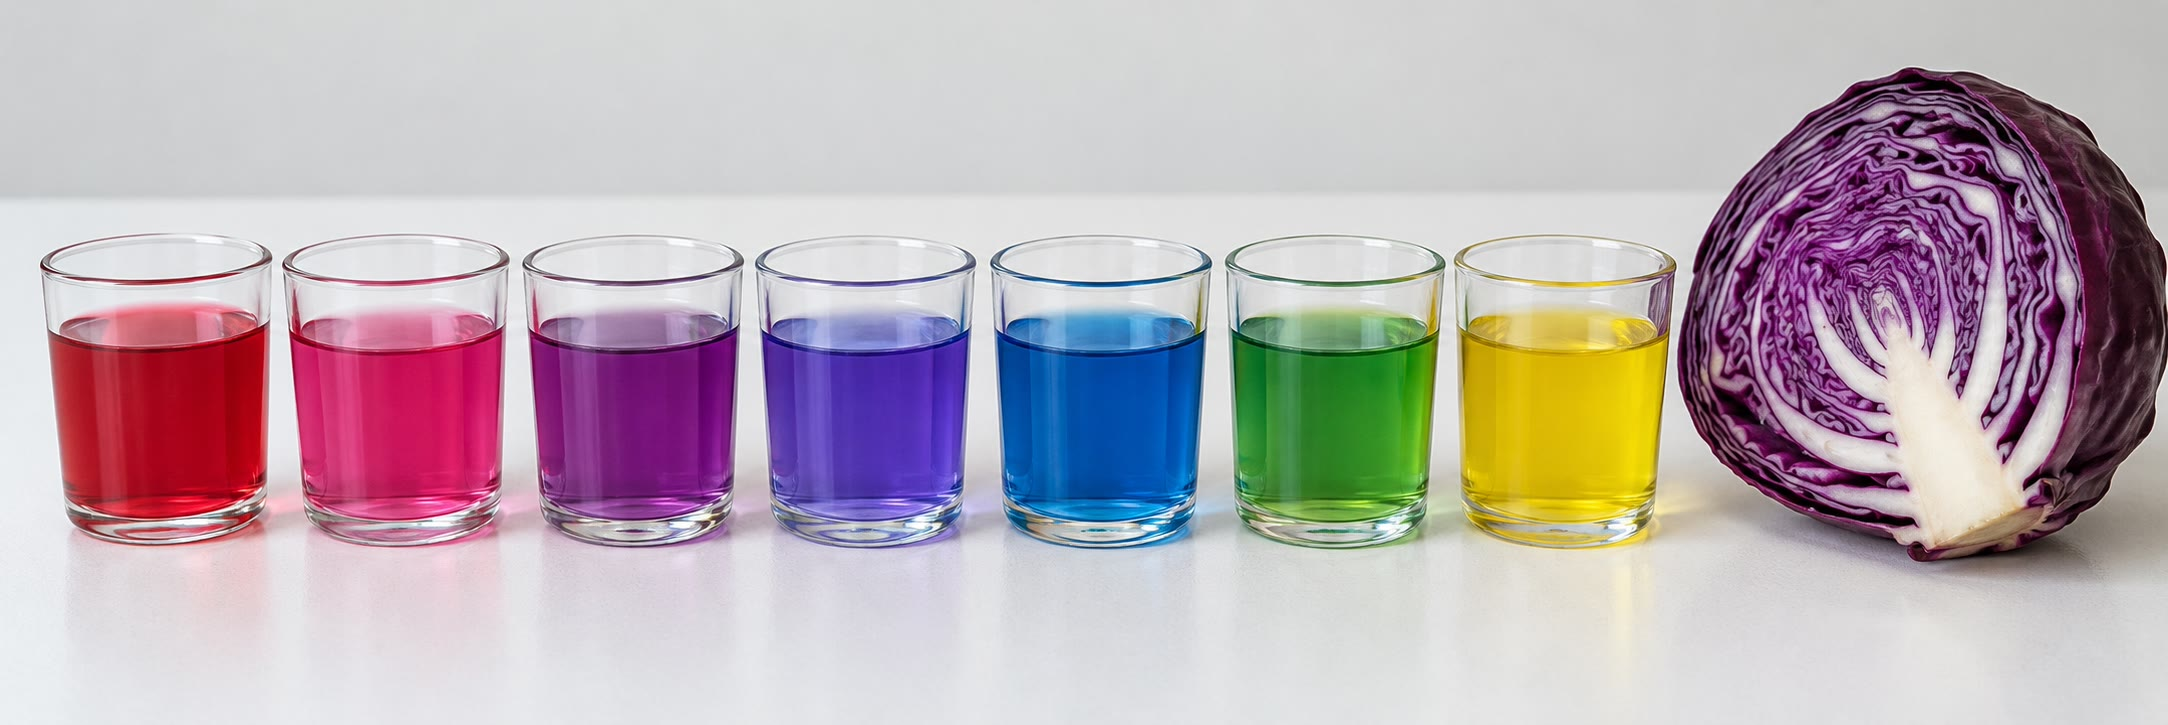
\includegraphics[width=0.55\linewidth]{images/book1/ai/g9-red-cabbage.jpg}

{\small Le jus de chou rouge, préparé par un enseignant, change de
couleur avec le \omterm{def:g9:acids-bases-ph:ph}{pH}~: rouge dans les acides, violet près de la
neutralité, puis bleu, vert et jaune dans des solutions de plus en plus
basiques.}
\end{omfigure}

\section{La sécurité avec les produits corrosifs}

\begin{safety}{\ghs[0.85cm]{GHS05}\ghs[0.85cm]{GHS07}}
% ledger: ghs:HCl, ghs:NaOH
L'acide chlorhydrique concentré et l'hydroxyde de sodium (la base des
déboucheurs) portent le pictogramme de corrosion GHS05~: ils provoquent
de graves brûlures de la peau et des yeux et attaquent les métaux.
GHS07~: irritant. Lunettes et gants~; une éclaboussure se rince aussitôt
à grande eau.
\end{safety}

\begin{remark}[Ne jamais mélanger les produits ménagers]\label{rem:g9:acids-bases-ph:mix}
Les produits acides et basiques réagissent entre eux, parfois
violemment, et certains \omterm{def:g6:pure-substances-and-mixtures:mixture}{mélanges} libèrent des gaz toxiques~: l'eau de
Javel mélangée à un détartrant acide dégage du dichlore. On ne \omterm{def:g6:pure-substances-and-mixtures:mixture}{mélange}
jamais les produits ménagers.
\end{remark}

\section{Exercices}

\begin{exercise}[$\star$]\label{exo:g9:acids-bases-ph:1}
Acide, basique ou neutre~? Une solution de \omterm{def:g9:acids-bases-ph:ph}{pH} 3, une de \omterm{def:g9:acids-bases-ph:ph}{pH} 7, une de
\omterm{def:g9:acids-bases-ph:ph}{pH} 11.
\end{exercise}

\begin{exercise}[$\star$]\label{exo:g9:acids-bases-ph:2}
Quels \omterm{def:g9:ions:ion}{ions} sont les plus nombreux dans une \omterm{def:g9:acids-bases-ph:acidic}{solution acide}~? Dans une
\omterm{def:g9:acids-bases-ph:acidic}{solution basique}~?
\end{exercise}

\begin{exercise}[$\star$]\label{exo:g9:acids-bases-ph:3}
À l'aide de l'échelle de \omterm{def:g9:acids-bases-ph:ph}{pH} de ce chapitre, range de la plus acide à la
plus basique~: le café, l'eau de mer, le jus de citron vert,
l'ammoniaque ménagère, l'eau pure.
\end{exercise}

\begin{exercise}[$\star$]\label{exo:g9:acids-bases-ph:4}
Décris comment mesurer le \omterm{def:g9:acids-bases-ph:ph}{pH} d'une solution avec du \omterm{def:g9:acids-bases-ph:ph-paper}{papier pH}.
\end{exercise}

\begin{exercise}[$\star\star$]\label{exo:g9:acids-bases-ph:5}
On dilue dix fois avec de l'eau une solution de \omterm{def:g9:acids-bases-ph:ph}{pH} 4. Quel est, environ,
son nouveau \omterm{def:g9:acids-bases-ph:ph}{pH}~? Et si on la dilue cent fois~?
\end{exercise}

\begin{exercise}[$\star\star$]\label{exo:g9:acids-bases-ph:6}
Une \omterm{def:g9:acids-bases-ph:acidic}{solution acide} peut-elle devenir basique si on lui ajoute de
l'eau~? Explique.
\end{exercise}

\begin{exercise}[$\star\star$]\label{exo:g9:acids-bases-ph:7}
Pourquoi faut-il verser l'acide dans l'eau, et non l'inverse~?
\end{exercise}

\begin{exercise}[$\star\star$]\label{exo:g9:acids-bases-ph:8}
Un flacon porte le pictogramme GHS05. Que signifie-t-il~? Donne deux
précautions.
\end{exercise}

\begin{exercise}[$\star\star$]\label{exo:g9:acids-bases-ph:9}
Combien de dilutions au dixième faut-il pour faire passer un acide de
\omterm{def:g9:acids-bases-ph:ph}{pH} 1 à \omterm{def:g9:acids-bases-ph:ph}{pH} 4~? Quelle est la dilution totale~?
\end{exercise}

\begin{exercise}[$\star\star$]\label{exo:g9:acids-bases-ph:10}
On prend du lait de magnésie contre l'acidité de l'estomac. Explique
pourquoi à l'aide de l'échelle de \omterm{def:g9:acids-bases-ph:ph}{pH}.
\end{exercise}

\begin{exercise}[$\star\star\star$]\label{exo:g9:acids-bases-ph:11}
Le \omterm{def:g9:acids-bases-ph:ph}{pH} de l'océan a baissé d'environ 0.1 depuis l'ère industrielle.
L'océan est-il acide aujourd'hui~? Dans quel sens évolue-t-il, et
pourquoi~?
\end{exercise}

\begin{exercise}[$\star\star\star$]\label{exo:g9:acids-bases-ph:12}
Un élève mesure le \omterm{def:g9:acids-bases-ph:ph}{pH} d'un même vinaigre avec du \omterm{def:g9:acids-bases-ph:ph-paper}{papier pH} (3) et avec
un \omterm{def:g9:acids-bases-ph:ph-paper}{pH-mètre} (2.6). Explique pourquoi les deux résultats diffèrent et
lequel est le plus précis.
\end{exercise}

\section{Problème~: la fuite d'acide}

\begin{problem}[{Problème du week-end --- un litre d'acide renversé dans
un évier de laboratoire, et pourquoi le diluer n'est pas la solution}]
\label{pb:g9:acids-bases-ph:1}
Un flacon contenant \qty{1}{L} d'acide chlorhydrique dilué, de \omterm{def:g9:acids-bases-ph:ph}{pH} 2,
se brise dans un évier de laboratoire. L'évacuation ne doit recevoir
aucune solution de \omterm{def:g9:acids-bases-ph:ph}{pH} inférieur à 5. On prendra la règle de ce
chapitre~: pour cet acide, chaque dilution au dixième augmente le \omterm{def:g9:acids-bases-ph:ph}{pH}
d'une unité.

\medskip
\noindent\textbf{Partie I --- L'acide.}
\begin{enumerate}
  \item La solution est-elle acide, neutre ou basique~? Quels \omterm{def:g9:ions:ion}{ions}
        contient-elle en plus grand nombre~?
  \item Quel pictogramme le flacon doit-il porter, et pourquoi~?
  \item L'enseignant mesure le \omterm{def:g9:acids-bases-ph:ph}{pH} avec un \omterm{def:g9:acids-bases-ph:ph-paper}{pH-mètre} plutôt qu'avec du
        \omterm{def:g9:acids-bases-ph:ph-paper}{papier pH}. Donne un avantage.
  \item Combien de fois plus d'\omterm{def:g9:ions:ion}{ions} \ce{H+} y a-t-il dans un litre à
        \omterm{def:g9:acids-bases-ph:ph}{pH} 2 que dans un litre à \omterm{def:g9:acids-bases-ph:ph}{pH} 3 du même acide~?
\end{enumerate}

\medskip
\noindent\textbf{Partie II --- Diluer.}
\begin{enumerate}[resume]
  \item Quel volume de solution obtient-on en diluant dix fois le litre
        d'acide~? Quel est son \omterm{def:g9:acids-bases-ph:ph}{pH}~?
  \item Combien de dilutions au dixième faut-il pour atteindre \omterm{def:g9:acids-bases-ph:ph}{pH} 5~?
  \item Quel volume total de solution cela ferait-il~?
  \item Une quantité d'eau, quelle qu'elle soit, pourrait-elle rendre la
        \omterm{def:g9:acids-bases-ph:acidic}{solution basique}~? Explique.
\end{enumerate}

\medskip
\noindent\textbf{Partie III --- Une meilleure méthode.}
L'enseignant ajoute plutôt, peu à peu, une solution d'une base jusqu'à
ce que le \omterm{def:g9:acids-bases-ph:ph-paper}{papier pH} indique 7~: les \omterm{def:g9:ions:ion}{ions} \ce{H+} de l'acide réagissent
avec les \omterm{def:g9:ions:ion}{ions} \ce{OH-} de la base.
\begin{enumerate}[resume]
  \item Écris l'équation de la réaction entre les \omterm{def:g9:ions:ion}{ions} \ce{H+} et
        \ce{OH-}.
  \item Pourquoi est-ce mieux que de diluer~?
  \item Nomme un produit basique de tous les jours qui pourrait servir
        dans une cuisine à nettoyer une petite flaque de vinaigre.
  \item Calcule le volume d'eau qu'il faudrait ajouter au litre d'acide
        pour l'amener à \omterm{def:g9:acids-bases-ph:ph}{pH} 5.
\end{enumerate}
\end{problem}
